\newpage
\section{Interface}
The interface gives the driver an opportunity to coomunicate with the system. This gives the driver some form of control over the operation of the vehicle. Furthermore it ensures the driver has the ability to use the horn and to keep the dead man safety switch activated as stated by the requirements.

The interface also includes the connections to the CAN-Transceiver and the SD-card, but these will be discussed in their own respective sections accordingly.
  
\subsection{Design}
The design consist of 2 connections for each button, with at pulldown resistor at each pin. This ensures no perception of a false positive at the MCU. As seen on the picture, the interface consists of 4 different buttons. These buttons are:

\begin{itemize}
	\item{Dead Man Safety Switch}
	\item{Start button for driving algorithm}
	\item{Stop button for driving algorithm}
	\item{Button for controlling the horn}
\end{itemize}

\begin{figure}[H]
	\centering
	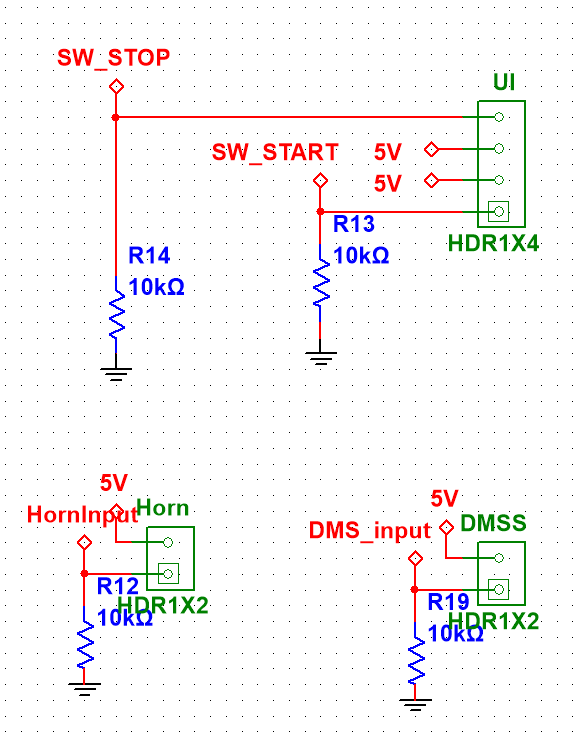
\includegraphics[width=0.6\linewidth]{Hardware/Pictures/User_interface}
	\caption{Interface circuit diagram}
	\label{fig:interface}
\end{figure}

\newpage
\subsection{Implementation}
The buttons will be placed inside the cockpit, which gives driver easy access to them. Since the requirements states that all electronic must be placed behind bulkhead, there must be run long wires from the casing to the buttons. The long wires are prone to noise induction, but this part have been overlooked. This can be done, since the signal running along the wires do not carry sensitive information in the sense that the MCU is indifferent of the voltage level as long as it upholds the limits of MCU.

There hasn't been any final decisions made for which buttons that is going to be implemented into the car to work as the interface. The demands for the button are not high and therefore the choice is open and is depedent on the amount of space given by the engineers building the car.

\subsection{Unity test}
The test is performed by placing the scope on either pin that is connected to a button.

The measurement equals a step input with a slight ripple due to bouncing of the button, which is removed internally in the MCU with a debouncer. 